%%%%%%
%
% PROJECT 3 - MODELING OIL PRODUCTION
%
% filename: modeling_oil_production.tex
% last modified: 2014-7-16
%
%%%%%%%
%
%
%%%%%%%

\documentclass
[justified,nohyper]
{tufte-handout}

\usepackage{booktabs}
\usepackage{graphicx}
\usepackage{kmath,kerkis} % The order of the packages matters; kmath changes the default text font
\usepackage[T1]{fontenc}

\begin{document}
\begin{center}
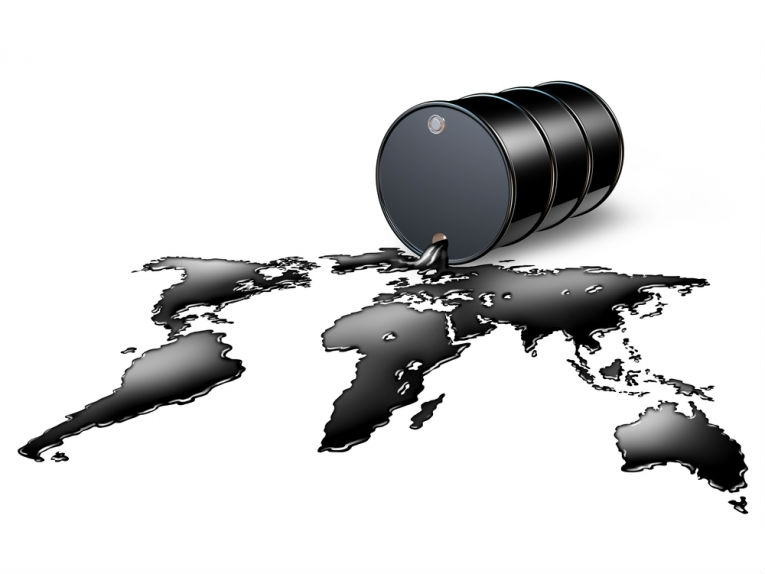
\includegraphics[scale=0.3]{oil.jpg}
\end{center}
\section{Advanced Calculus Project 3: Modeling World Oil Production}
\newthought{There are two things} that are clear about crude oil. One is that we use a lot of it. The world consumption of crude oil is approximately 80 million barrels per day, and world consumption grew by 3.4\% in 2004.\sidenote{\textit{New Scientist}, 21 May 2005, page 7.}

The other is that the Earth's oil reserves are finite. The processes that created crude oil that we use today are fairly well understood. There may be significant deposits of crude oil yet to be discovered, but it is a limited resource.

Governments, economists, and scientists argue endlessly about almost every other aspect of oil production. Exactly how much oil is left in the Earth and what fraction of that oil can or will ever be removed is difficult to estimate and has significant financial ramifactions. Substantial disagreement on oil policy is not surprising.

Predictions of the decline in production are notoriously difficult, and it is easy to find examples of such predictions that ended up being absurdly wrong.\sidenote{For example, http://goo.gl/Yunzsk} On the other hand, sometimes predictions of decline in production are accurate. In \textit{Hubbert's Peak}\sidenote{Deffeyes, K.S., \textit{Hubbert's Peak}, Princeton University Press, Princeton and Oxford, 2001.}, Kenneth Deffeyes recounts the work of geologist M. King Hubbert. Hubbert fit a logistic model, precisely the type we have been looking at for things like population growth, to the production data for crude oil in the United States. Using production data up to the mid 1950s along with approximations of the total amount of recoverable crude oil, Hubbert predicted that production would peak in the U.S. in the 1970s. He was right.

\newthought{In this project} you will model the U.S. and world crude oil production using a logistic model, where the carrying capacity represents the total possible recoverable crude oil. Your final report should address the following items:

\begin{enumerate}
  \item Find parameter values for a logistic differential equation that fit the crude oil production data for the U.S. (see Table \ref{oil1}).\sidenote{Data from Twentieth Century Petroleum Statistics, 1984, by DeGolyer and MacNaughton and http://www.eia.doe.gov}
  \item Predicting both the growth rate and the total amount of recoverable crude oil from the data is difficult. Model the crude oil production of the U.S. assuming the total amount of recoverable crude oil in the U.S. is 200 billion barrels. (This assumption includes what has already been recovered and serves the role of the carrying capacity in the logistic model.)
  \item Repeat Part 2 replacing 200 billion barrels with 300 billion barrels.
  \item Model the world crude oil production based on estimates of total recoverable crude oil (past and future) of 2.1 trillion barrels and 3 trillion barrels. (Both of these estimates are commonly used. They are based on differing assumptions concerning what it means for crude oil to be ``recoverable.'') When do the models predict that the rate of production of oil reaches its maximum?
  \item The decline in production of crude oil will certainly result in an increase in price of oil products. This price increase will provide more funds for crude oil production, perhaps slowing the rate of decline. Describe how this price increase might affect the predictions of your model for world oil production and how you might modify your model to reflect these assumptions.
\end{enumerate}

\textbf{Your report:} As always, your report needs an abstract and conclusion with sufficient explanation of what you did to solve this problem. Please present your models one at a time, with separate explanations of each. Discuss how well they fit the data and how sensitive this fit is to small changes in the parameters. As the title of this project suggests, you will need to come to some conclusion about when the ``peak'' occurs and how long we have until the oil ``runs out.'' Both of these dates should be clear from reading your report and should be supported by your mathematical analysis. 

\begin{fullwidth}
\begin{table}
\begin{tabular}{ccc||ccc}
\toprule
Year & U.S. Oil & World Oil & Year & U.S. Oil & World Oil \\
\midrule
1920-24 & 2.9 & 4.3 & 1970-74 & 17.0 & 93.9 \\
1925-29 & 4.2 & 6.2 & 1975-79 & 15.3 & 107 \\
1930-34 & 4.3 & 7.0 & 1980-84 & 15.8 & 101 \\
1935-39 & 5.8 & 9.6 & 1985-89 & 15.2 & 104 \\
1940-44 & 7.5 & 11.3 & 1990-94 & 12.9 & 110 \\
1945-49 & 9.2 & 15.2 & 1995-99 & 11.5 & 118 \\
1950-54 & 11.2 & 22.4 & 2000-04 & 10.4 & 126 \\
1955-59 & 12.7 & 31.9 & 2005-09 & 9.3 &  130\\
1960-64 & 13.4 & 44.6 & 2010-12 & 6.4 &  80.5 \\
1965-69 & 15.8 & 65.4 &         &     &     \\
\bottomrule
\caption{\label{oil1} Oil production per five year periods in billions of barrels}
\end{tabular}
\end{table}
\end{fullwidth}

\end{document}